\documentclass[final]{beamer}

\mode<presentation>{
    \usetheme{UCB}
}
\usepackage{amsmath,amsthm, amssymb, latexsym}
\usepackage{graphicx}
\usepackage{epstopdf}

\boldmath
\usepackage[english]{babel}
\usepackage[latin1]{inputenc}

\usepackage[orientation=landspace,size=custom,height=76.2,width=101.6,scale=1.4,debug]{beamerposter}

\usepackage{listings}
%\lstloadlanguages{Haskell}
%\lstnewenvironment{code}
    %{\lstset{}%
      %\csname lst@SetFirstLabel\endcsname}
    %{\csname lst@SaveFirstLabel\endcsname}
    %\lstset{
      %basicstyle=\small\ttfamily,
      %flexiblecolumns=false,
      %basewidth={0.5em,0.45em},
      %literate={+}{{$+$}}1 {/}{{$/$}}1 {*}{{$*$}}1 {=}{{$=$}}1
               %{>}{{$>$}}1 {<}{{$<$}}1 {\\}{{$\lambda$}}1
               %{\\\\}{{\char\char}}1
               %{->}{{$\rightarrow$}}2 {>=}{{$\geq$}}2 {<-}{{$\leftarrow$}}2
               %{<=}{{$\leq$}}2 {=>}{{$\Rightarrow$}}2 
               %{\ .}{{$\circ$}}2 {\ .\ }{{$\circ$}}2
               %{>>}{{>>}}2 {>>=}{{>>=}}2
               %{|}{{$\mid$}}1               
    %}

\definecolor{gray_ulisses}{gray}{0.55}
\definecolor{castanho_ulisses}{rgb}{0.71,0.33,0.14}
\definecolor{preto_ulisses}{rgb}{0.41,0.20,0.04}
\definecolor{green_ulises}{rgb}{0.2,0.75,0}


\lstdefinelanguage{HaskellUlisses} {
    basicstyle=\ttfamily\small,
    sensitive=true,
    morecomment=[l][\color{gray_ulisses}\ttfamily\tiny]{--},
    morecomment=[s][\color{gray_ulisses}\ttfamily\tiny]{\{-}{-\}},
    morestring=[b]",
    stringstyle=\color{red},
    showstringspaces=false,
    numberstyle=\tiny,
    numberblanklines=true,
    showspaces=false,
    breaklines=true,
    showtabs=false,
    emph=
    {[1]
        FilePath,IOError,abs,acos,acosh,all,and,any,appendFile,approxRational,asTypeOf,asin,
        asinh,atan,atan2,atanh,basicIORun,break,catch,ceiling,chr,compare,concat,concatMap,
        const,cos,cosh,curry,cycle,decodeFloat,denominator,digitToInt,div,divMod,drop,
        dropWhile,either,elem,encodeFloat,enumFrom,enumFromThen,enumFromThenTo,enumFromTo,
        error,even,exp,exponent,fail,filter,flip,floatDigits,floatRadix,floatRange,floor,
        fmap,foldl,foldl1,foldr,foldr1,fromDouble,fromEnum,fromInt,fromInteger,fromIntegral,
        fromRational,fst,gcd,getChar,getContents,getLine,head,id,inRange,index,init,intToDigit,
        interact,ioError,isAlpha,isAlphaNum,isAscii,isControl,isDenormalized,isDigit,isHexDigit,
        isIEEE,isInfinite,isLower,isNaN,isNegativeZero,isOctDigit,isPrint,isSpace,isUpper,iterate,
        last,lcm,length,lex,lexDigits,lexLitChar,lines,log,logBase,lookup,map,mapM,mapM_,max,
        maxBound,maximum,maybe,min,minBound,minimum,mod,negate,not,notElem,null,numerator,odd,
        or,ord,otherwise,pi,pred,primExitWith,print,product,properFraction,putChar,putStr,putStrLn,quot,
        quotRem,range,rangeSize,read,readDec,readFile,readFloat,readHex,readIO,readInt,readList,readLitChar,
        readLn,readOct,readParen,readSigned,reads,readsPrec,realToFrac,recip,rem,repeat,replicate,return,
        reverse,round,scaleFloat,scanl,scanl1,scanr,scanr1,seq,sequence,sequence_,show,showChar,showInt,
        showList,showLitChar,showParen,showSigned,showString,shows,showsPrec,significand,signum,sin,
        sinh,snd,span,splitAt,sqrt,subtract,succ,sum,tail,take,takeWhile,tan,tanh,threadToIOResult,toEnum,
        toInt,toInteger,toLower,toRational,toUpper,truncate,uncurry,undefined,unlines,until,unwords,unzip,
        unzip3,userError,words,writeFile,zip,zip3,zipWith,zipWith3,listArray,doParse
    },
    emphstyle={[1]\color{blue}},
    emph=
    {[2]
        Bool,Char,Double,Either,Float,IO,Integer,Int,Maybe,Ordering,Rational,Ratio,ReadS,ShowS,String,
        Word8,InPacket
    },
    emphstyle={[2]\color{castanho_ulisses}},
    emph=
    {[3]
        case,class,data,deriving,do,else,if,import,in,infixl,infixr,instance,let,
        module,of,primitive,then,type,where
    },
    emphstyle={[3]\color{preto_ulisses}\textbf},
    emph=
    {[4]
        quot,rem,div,mod,elem,notElem,seq
    },
    emphstyle={[4]\color{castanho_ulisses}\textbf},
    emph=
    {[5]
        EQ,False,GT,Just,LT,Left,Nothing,Right,True,Show,Eq,Ord,Num
    },
    emphstyle={[5]\color{preto_ulisses}\textbf}
}


\lstnewenvironment{code}%
{\lstset{language=HaskellUlisses}}%
{}%


\usepackage{array,booktabs,tabularx}

\newcolumntype{Z}{>{\centering\arraybackslash}X} % centered tabularx columns
\newcolumntype{V}{>{\centering\arraybackslash} m{.3\linewidth} }
\newcommand{\pphantom}{\textcolor{ta3aluminium}} % phantom introduces a vertical space in p formatted table columns??!!

\listfiles


\setbeamertemplate{caption}[numbered]



\title{\huge HasView}
\subtitle{\LARGE A Visual Haskell Editor}
\institute{University of California at Berkeley}
\author{Brandon Wang and Kaushik Iyer}
\date{9 May, 2011}

\newlength{\columnheight}
\setlength{\columnheight}{105cm}


\begin{document}
\begin{frame}[fragile]
    \begin{columns}[T]
        \begin{column}{.3\textwidth}
            \begin{beamercolorbox}[wd=\textwidth]{postercolumn}
                    %\parbox[t][\columnheight]{\textwidth}{ % must be some better way to set the the height, width and textwidth simultaneously
                % Since all columns are the same length, it is all nice and tidy.  You have to get the height empirically
                % ---------------------------------------------------------%
                % fill each column with content            
                        \begin{block}{Introduction}
                            \begin{itemize}
                                \item A system that allows \alert{visual} Haskell programming
                                \item Use ideas from \alert{dataflow programming}:
                                    \begin{itemize}
                                        \item functions $\mapsto$ blocks
                                        \item recursion $\mapsto$ nesting
                                        \item control flow $\mapsto$ arrows
                                    \end{itemize}
                                \item Requirements:
                                    \begin{description}
                                        \item[Extensible] \hfill Need to be able to easily write new structures --- use Python
                                        \item[Modular] \hfill Class based structure to allow for abstraction of GUI elements
                                        \item[Compilation] \hfill Need to be able to compile to GHC-compatible Haskell
                                    \end{description}
                            \end{itemize}
                        \end{block}
                \begin{block}{Serialization}
                    \begin{figure}
                        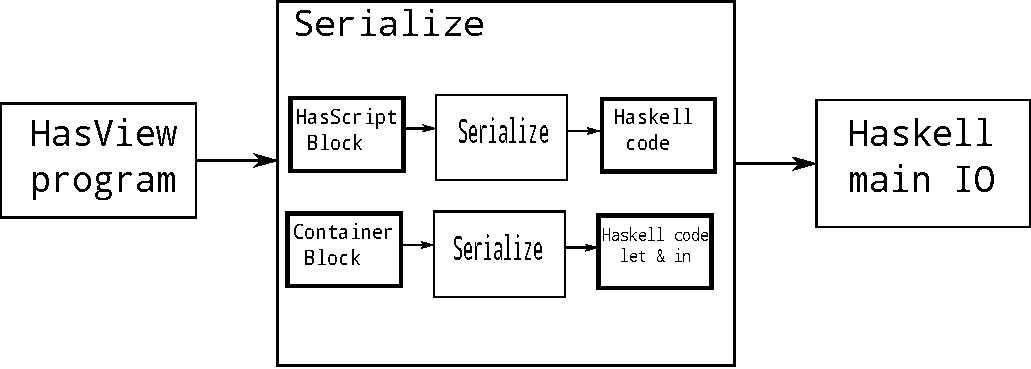
\includegraphics[width=1\textwidth]{serialize.pdf}
                    \end{figure}
                \end{block}

                        
                    %}


                \begin{block}{Serialization and Resolution Example}
                    \begin{figure}
                        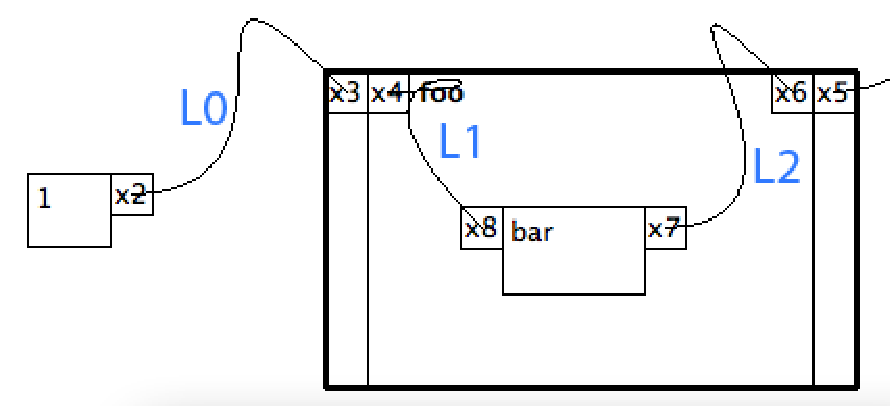
\includegraphics[width=0.7\textwidth]{resolution-raw.pdf}
                    \end{figure}
                \end{block}
                \begin{block}{Serialization and Resolution Explanation}
                    \begin{figure}
                        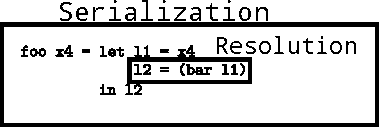
\includegraphics[width=0.9\textwidth]{resolution.pdf}
                    \end{figure}
                \end{block}

            \end{beamercolorbox}


        \end{column}

        \begin{column}{.35\textwidth}
            \begin{beamercolorbox}[wd=\textwidth]{postercolumn}
                %\begin{minipage}[T]{.95\textwidth}  % tweaks the width, makes a new \textwidth
                    %\parbox[t][\columnheight]{\textwidth}{ % must be some better way to set the the height, width and textwidth simultaneously
                % Since all columns are the same length, it is all nice and tidy.  You have to get the height empirically
                % ---------------------------------------------------------%
                % fill each column with content            
                \begin{block}{Calculating \texttt{fib}}
                    \begin{figure}
                        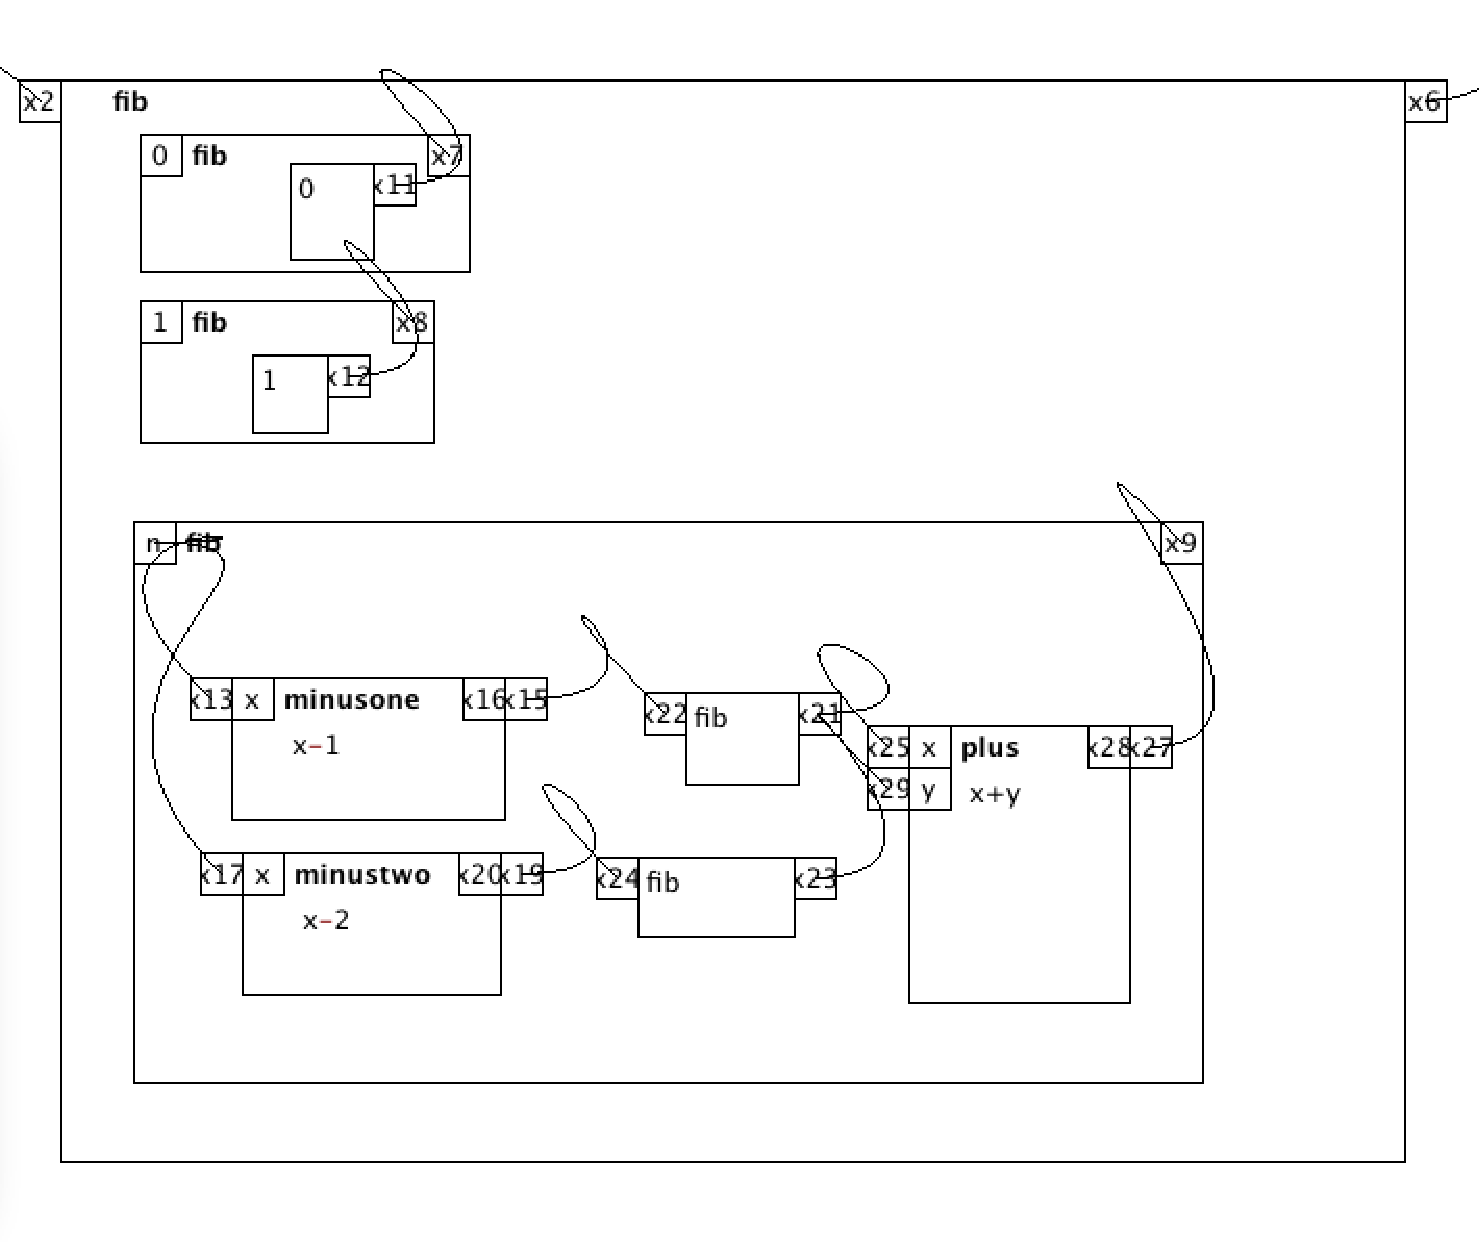
\includegraphics[width=1\textwidth]{fib-diagram.pdf}
                    \end{figure}
                \end{block}
                \begin{block}{Calculating \texttt{map}}
                    \begin{figure}
                        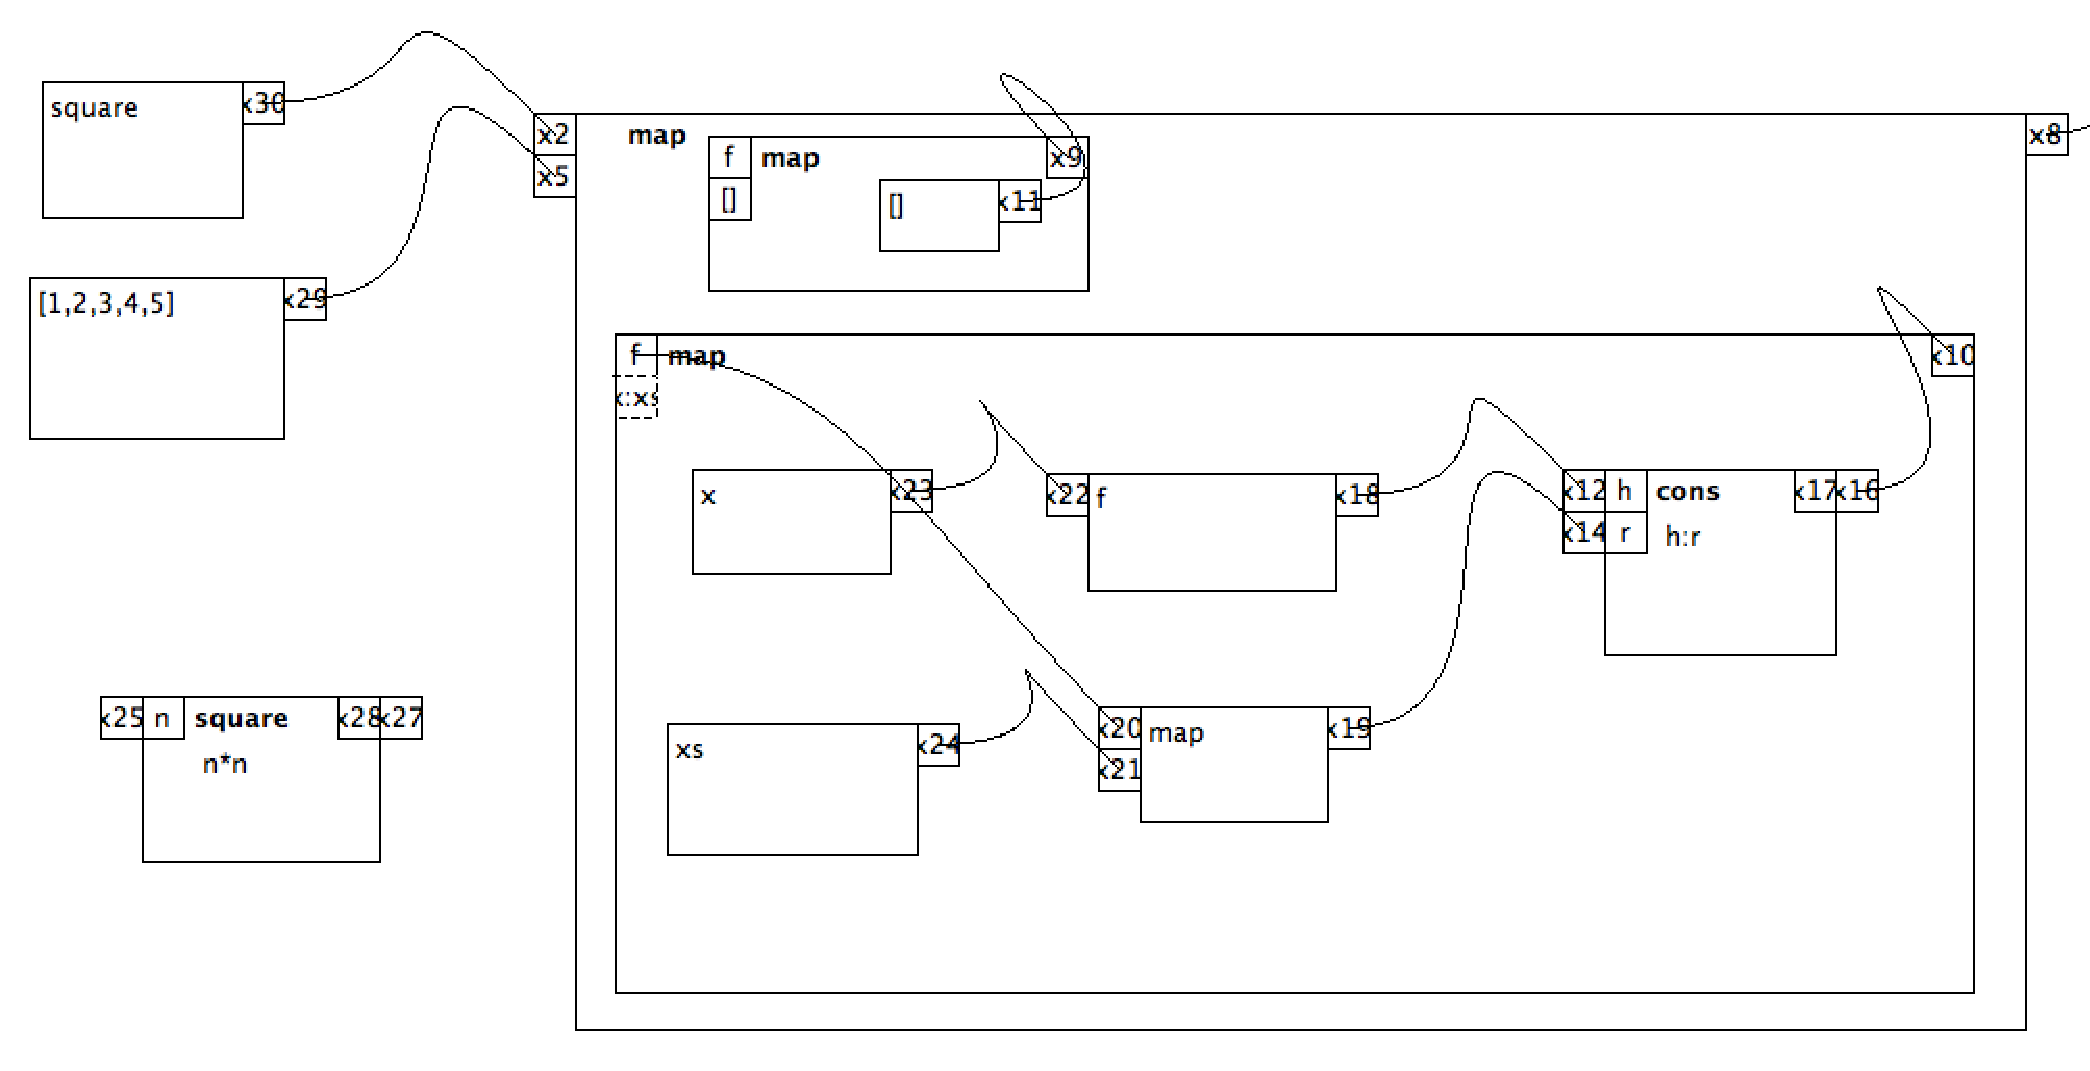
\includegraphics[width=1\textwidth]{map-diagram.pdf}
                    \end{figure}
                \end{block}
            \end{beamercolorbox}
        \end{column}

        \begin{column}{.31\textwidth}
            \begin{beamercolorbox}[wd=\textwidth]{postercolumn}
                \begin{block}{Compiled \texttt{fib} code}
                    \begin{code}
main = let fib 0 = let l1 = 0
                    in l1
            fib 1 = let l2 = 1
                    in l2
            fib n = let l6 = n
                        l7 = n
                        minustwo x = x - 2
                        l12 = plus l10 l11
                        minusone x = x - 1
                        plus x y = x + y
                        l10 = (fib 18)
                        l11 = (fib 19)
                        l8 = minusone l6
                        l9 = minustwo l7
                    in l12
            l0 = fib l13
            l13 = 25
        in print l0
                    \end{code}
                \end{block}

                \begin{block}{Compiled \texttt{map} code}
                    \begin{code}
main = let l10 = map  l9 l8
           map  f [] = let l0 = []
                       in l0
           map  f (x:xs) = let l6 = (map  l5 l4)
                               l7 = cons  l3 l6
                               l4 = xs
                               l5 = f
                               l2 = x
                               l3 = (f  l2)
                               cons  h r = h:r
                           in l7
           square n = n*n
           l8 = [1,2,3,4,5]
           l9 = square
       in print l10
                    \end{code}
                \end{block}
       \end{beamercolorbox}
                            \vfill
       \end{column}
                                %}
                            %\end{minipage}
    \end{columns}
  %\vskip1ex
  %\tiny\hfill{Created with \LaTeX \texttt{beamerposter}  \url{http://www-i6.informatik.rwth-aachen.de/~dreuw/latexbeamerposter.php} \hskip1em}
\end{frame}
\end{document}
